\section{Introduction}

When connecting two rotary mechanical devices a coupler is used. These include the use of 1:1 flexible shaft couplers, to compensate for possible shaft misalignments, as well as belts, and gear boxes. In theory it is desired to have the given coupler be perfectly rigid, every degree the actuator turns the connected load will turn to its precise location denoted by the input and the gear ratio. For a coupler to be perfectly rigid the latter must be true for all time. In reality gear boxes and couplers are not perfectly rigid and have spring and damping terms associated with them. The spring constant causes the system to have two resonant frequencies collectively called the Torsional Resonance (TR). The TR frequencies, which are referred to as the resonant frequency, $\omega_r$, and the anti-resonant frequency, $\omega_{ar}$, can not fall within the pass-band of the closed loop servo because it will cause instability.  Fig.~\ref{fig:couple} shows a diagram of a coupled system exhibiting TR. The ideal system can be reduced to a single acting inertia of $J_a+J_L$ while the system exhibiting TR is connected by a spring damper system thus that reduction can not be made.  Our goal is to demonstrate a controller that uses commonly measured states (such as motor position) to reduce the effects of TR on coupled systems.

\begin{figure}[t]
  \centering
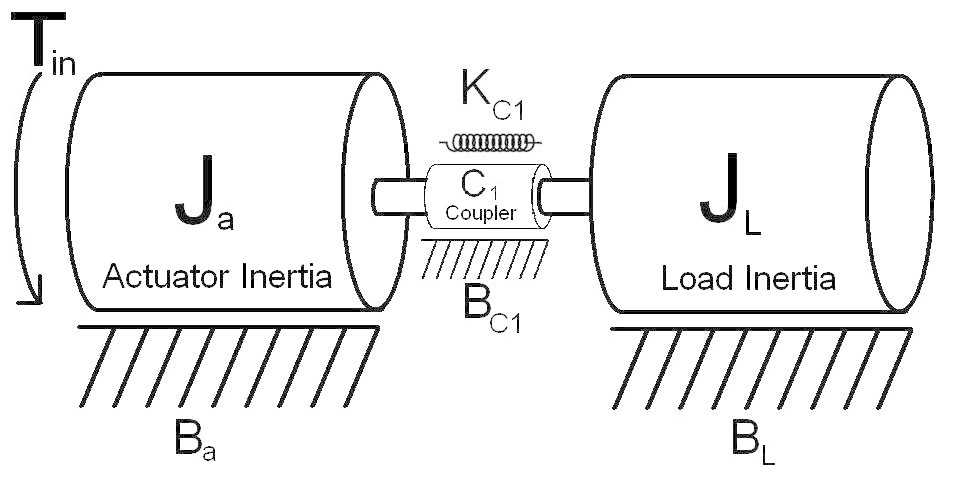
\includegraphics[width=1.0\columnwidth]{./pix/couple.png}
  \caption{System exhibiting TR. In an ideal
system (without TR) the load can be represented as a single acting inertia $(J_a+J_L)$.  The system exhibiting TR is connected by a
spring damper system thus that reduction can not be mad}
  \label{fig:couple}
\end{figure}

In this paper 
Section~\ref{sec:back} gives a brief overview of TR and the contemporary ways of reducing its effects.
Section~\ref{sec:trModel} models a system exhibiting TR. 
Section~\ref{sec:load} shows the effects of TR on the system.
Section~\ref{sec:meth} goes through two method of reducing the effects of TR (one linear and one non-linear method) where
Section~\ref{sec:re} demonstrates a linear method based on state feedback by Rizzo et. al. and
Section~\ref{sec:smc} demonstrates a non-linear sliding-mode control based method.
Section~\ref{sec:con} show and discusses the results of both methods and gives final thoughts.


